\section{PS1b: PhotoMagic}\label{sec:ps1b}
\graphicspath{{ps1b}}
\subsection{Discussion:}\label{sec:ps1b:disc}
The ps1b utilizes the ps1a i.e \textbf{LFSR: LINEAR FEEDBACK SHIFT REGISTER} as a supporting for the encoding and decoding of the image given as input.This project takes the input image i.e, Cat.png and Encrypts using the LFSR Randomizer and encrypts each and every pixel
of the image and saves to the cat-out.png file.
   For Encryption I used Common Example i.e; \newline
    \colorbox{yellow}{\textbf{./PhotoMagic cat.png cat-out.png 0011001100000 8}} \newline
    \textbf{Figure:\ref{fig:encode}} \newline
If we want to decrypt the encrypted image we write it as follows. \newline
    \colorbox{yellow}{\textbf{./PhotoMagic cat-out.png cat.png 0011001100000 8}} \newline
     \textbf{Figure: \ref{fig:decode}}
    
\subsection{Key algorithms, Data structures and OO Designs used in this Assignment:}\label{sec:ps1b:kdo}

I used The Vector STL in the LFSR as it is much easier to use and I felt flexible in it. Also Improvised the sample code to the Final code to get the perfect output. I used Image and its funtions and letter sent to Texture then to Sprite to draw on the window I used Two windows and two sprites for showing the difference between the normal cat image and the encoded and decoded image. The following code is used for the encoding and decoding: \newline
 \begin{lstlisting}
 void transform(sf::Image& kitty_image, FibLFSR* fibo){
	sf::Vector2u size = kitty_image.getSize();
	sf::Color color, newColor;

	for(int i = 0; i < size.x; i++){
		for(int j = 0; j < size.y; j++){
			color = kitty_image.getPixel(i, j);

			color.r = color.r xor fibo->generate(8);
			color.g = color.g xor fibo->generate(8);
			color.b = color.b xor fibo->generate(8);

			kitty_image.setPixel(i, j, color);	
		}
	}
}
 \end{lstlisting}

\subsection{Images used:}\label{sec:ps1b:img}
\begin{figure}[h]
    \centering
    
\includegraphics[width=0.45\textwidth]{ps1b/cat.png}
    \caption{Cat Image}
    \label{fig:mesh1}
\end{figure}


\subsection{What I accomplished :}\label{sec:ps1b:accomplish}

I accomplished the Encoding and Decoding of the Image using the C++ language in an efficient way. I have achieved using multiple windows, which was an amazing thing to do. 

\subsection{What I already knew :}\label{sec:ps1b:knew}

I knew how to take the input of the file and write to an output file. I already knew about how to create sprite using images and texture. I also knew how to display the windows and also to create the Makefile for the project.

\subsection{What I learned :}\label{sec:ps1b:learn}

I learned how to utilize two windows for the different output. I understood the concept of encoding and decoding using the pixels of the image and using the LFSR Randomizer. I also got to know about the mathematical calculations for the pixels.

\subsection{Challenges :}\label{sec:ps1b:challenges}

To find out the image pixels and the also to identify how to tranform them to the normal to encoded and then decode the image.

\subsection{Acknowledgements :}\label{sec:ps1b:ack}
\begin{itemize}
    \item \url{https://www.sfml-dev.org/tutorials/2.5/}
\end{itemize}
\newpage

\subsection{Codebase}\label{sec:ps1b:code}

\colorbox{pink}{\textbf{Makefile:}} \newline \textbf{This Makefile is contains no lint but it includes the flags as well as it is extension of the ps1a Makefile.}

\lstinputlisting[language=Make]{ps1b/Makefile}

\colorbox{pink}{\textbf{PhotoMagic.cpp:}} \newline \textbf{This file is the main file where the reading and writing also the encoding and decoding of the image takes place. This file gives the output in two windows. Input window and output window of the file.}
\lstinputlisting{ps1b/PhotoMagic.cpp}

\colorbox{pink}{\textbf{PhotoMagic.h:}}
\newline \textbf{This file contains the initializations and header files for the PhotoMagic.cpp}
\lstinputlisting{ps1b/PhotoMagic.h}
\newpage

\colorbox{pink}{\textbf{test.cpp:}}
\newline

\textbf{Given test file for the ps1a Assignment.}
\lstinputlisting{ps1b/test.cpp}

\newpage
\subsection{Output:}\label{sec:ps1b:output}
\begin{figure}[h]
    \centering
    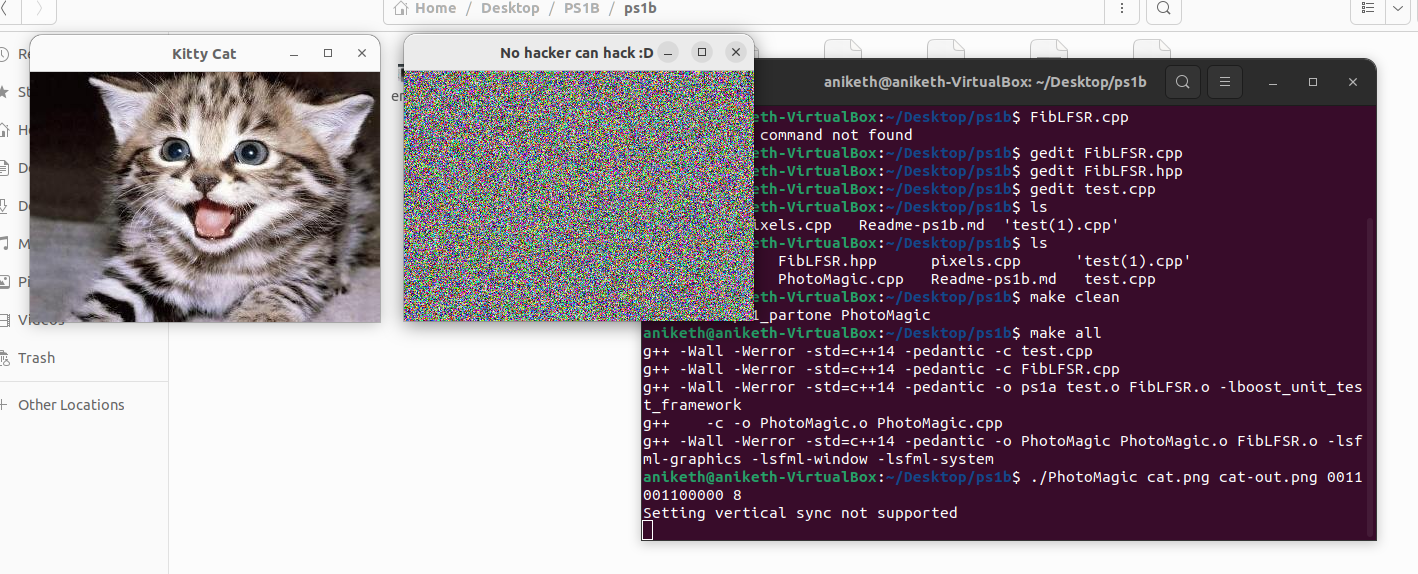
\includegraphics[width=1\textwidth]{ps1b/Encoded.png}
    \caption{Encoded Image}
    \label{fig:encode}
\end{figure}
\begin{figure}[h]
    \centering
    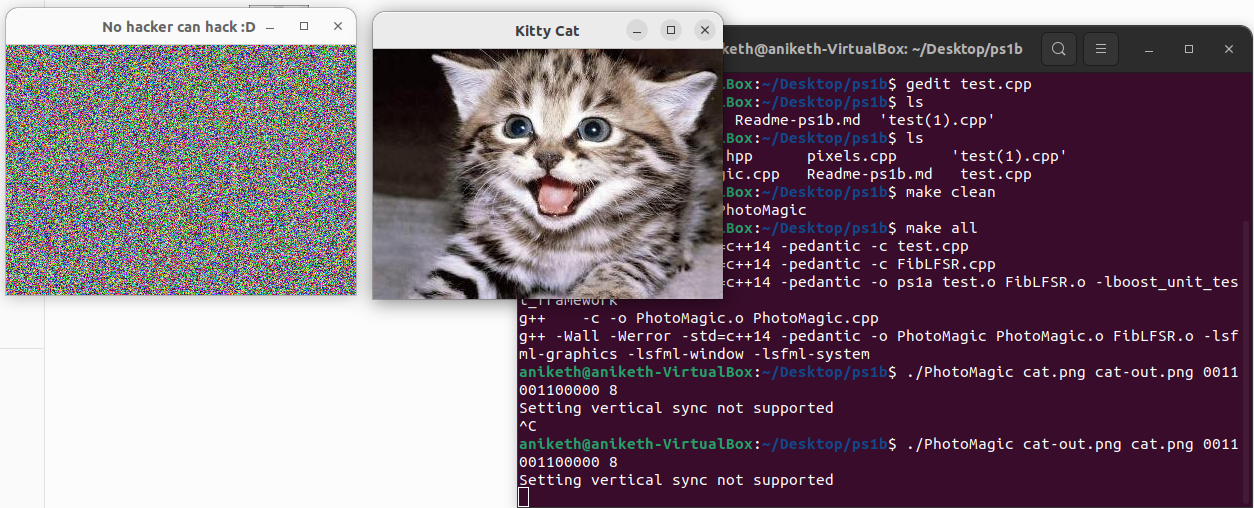
\includegraphics[width=1\textwidth]{ps1b/Decoded.png}
    \caption{Decode Image}
    \label{fig:decode}
\end{figure}


\newpage
